\documentclass[a4paper,12pt,onecolumn]{article}

\usepackage[utf8]{inputenc}
\usepackage[english]{babel}
\usepackage[T1]{fontenc}
\usepackage{lmodern}
\usepackage{amssymb,amsmath,amsthm,array,epsfig,pstricks,subfig,hyperref,verbatim}

\newtheorem{thm}{Theorem}
\newtheorem{lem}[thm]{Lemma}
\newtheorem{rem}[thm]{Remark}

\newenvironment{keywords}{{\upshape\bfseries Key words. }\ignorespaces}{}

\newcommand{\R}{{\mathbb R}}
\newcommand{\vol}{\mathcal{L}^d}
\newcommand{\dH}[1]{\;{\rm d}{\cal H}^{#1}} % Hausdorff measure
\newcommand{\dL}[1]{\;{\rm d}{\cal L}^{#1}} % Lebesgue measure
\newcommand{\bigchi}{\ensuremath{\mathrm{\mathcal{X}}}}
\newcommand{\charfcn}[1]{\bigchi_{#1}} % characteristic function
\newcommand{\Vh}{\underline{V}(\Gamma^m)}
\newcommand{\Wh}{W(\Gamma^m)}
\newcommand{\Vht}{\underline{V}(\Gamma^h(t))}
\newcommand{\Wht}{W(\Gamma^h(t))}
\newcommand{\uspace}{\mathbb{U}}
\newcommand{\pspace}{\mathbb{P}}
\newcommand{\kspace}{\mathbb{K}}
\newcommand{\xspace}{\mathbb{X}}
\newcommand{\sigmaO}{o}
\newcommand{\nabs}{\nabla_{\!s}}
\newcommand{\id}{\rm id}
\newcommand{\ddt}{\frac{\rm d}{{\rm d}t}}
\newcommand{\NbulkT}{\vec{N}_{\Gamma,\Omega}^T}
\newcommand{\Nbulk}{\vec{N}_{\Gamma,\Omega}}
\newcommand{\errorXx}{\|\Gamma^h - \Gamma\|_{L^\infty}}
\newcommand{\LerrorUu}[1]{\|\vec U - I^h_{#1}\,\vec u\|_{L^2}}
\newcommand{\HerrorUu}[1]{\|\vec U - I^h_{#1}\,\vec u\|_{H^1}}
\newcommand{\LerrorPp}{\|P - p\|_{L^2}}
\newcommand{\unitn}{\vec{\rm n}}
\newcommand{\mat}[1]{\underline{\underline{#1}}\rule{0pt}{0pt}}
\newcommand{\strikec}{\mbox{$c\!\!\!\!\:/$}}
\newcommand{\Mloss}{\mathcal{L}_{\rm loss}}
\newcommand{\ek}{e}

\renewcommand{\theequation}{\arabic{section}.\arabic{equation}}

\textwidth 425pt

\title{Fitted Finite Element Discretization of \\ Two-Phase Navier-Stokes 
Flow}
\author{Marco Agnese and Robert N\"urnberg%
\thanks{email: \texttt{\{m.agnese13,robert.nurnberg\}@imperial.ac.uk}}\\
\small
Department of Mathematics, Imperial College, London, SW7 2AZ, U.K.}
\date{}

\begin{document}

\captionsetup[subfigure]{labelformat=empty} % remove label subplot

\maketitle

\begin{abstract}
We propose a novel fitted finite element method for two-phase Navier-Stokes
flow problems that uses piecewise linear finite elements to approximate the
moving interface. We present several numerical experiments for our numerical 
method, which demonstrate the accuracy and robustness of the proposed algorithm.
\end{abstract}

\begin{keywords}
viscous incompressible two-phase flow, Navier-Stokes equations,
free boundary problem, surface tension, finite elements, front tracking
\end{keywords}

\setcounter{equation} 0
\section{Numerical results} \label{sec:numerical_results}
Throughout this section we use uniform time steps $\tau_m=\tau$, $m=0,\ldots, 
M-1$. In addition, we set $\vec U^0 = \vec 0$. 

The CPU times which we report are measured in seconds and correspond to a 
single thread computation on an Intel Xeon E5640 (2.67GHz) processor with 16 GB 
of main memory.

We define the following benchmark quantities for the continuous solution $(\vec 
u, p, \Gamma)$ of 
(\ref{eq:2a}--h). 
Let $y_c(t) = \int_{\Omega_-(t)} x_2 \dL2 / \mathcal{L}^2(\Omega_-(t))$ denote
the $x_2$-component of the bubble's centre of mass. Let $\strikec(t)$ denote 
the ``degree of circularity'' of $\Gamma(t)$, which is defined as the ratio of
the perimeter of an area-equivalent circle and $\mathcal{H}^{1}(\Gamma(t))$. 
Finally, let 
$V_c(t) = \int_{\Omega_-(t)} u_2(t) \dL2 / \mathcal{L}^2(\Omega_-(t))$ 
denote the bubble's rise velocity, where 
$\vec u(\cdot,t) = (u_1(\cdot,t),u_2(\cdot,t))^T$. 
In this paper, we use the following discrete approximations of
these benchmark quantities:
\begin{equation}
y_c^m = \frac1{\mathcal{L}^2(\Omega_-^m)}\,\int_{\Omega_-^m} x_2 \dL2\,,
\end{equation}
\begin{equation}
\strikec^m = 
\frac{\pi^{\frac{1}{d}}[2\,d\,\mathcal{L}^d(\Omega_-^m)]^\frac{d-1}{d}}
{\mathcal{H}^{d-1}(\Gamma^m)}\,,
\end{equation}
\begin{equation}
V^m_c = \frac{(\rho^m_-\,U^m_2, 1)}{(\rho^m_-,1)}\,.
\end{equation}

\subsection{2d benchmark problem 1} \label{sec:2d_benchmark_1}
We use the setup described in \cite{HysingTKPBGT09}, see Figure~2 there;
i.e.\ $\Omega = (0,1) \times (0,2)$ with 
$\partial_1\Omega = [0,1] \times \{0,2\}$ and 
$\partial_2\Omega = \{0,1\} \times (0,2)$.
Moreover, $\Gamma_0 = \{\vec z \in \R^2 : |\vec z - (\frac12, \frac12)^T| =
\frac14\}$.
The physical parameters from the test case 1 in \cite[Table~I]{HysingTKPBGT09} 
are then given by
\begin{equation} \label{eq:Hysing1}
\rho_+ = 1000\,,\quad \rho_- = 100\,,\quad \mu_+ = 10\,,\quad \mu_- = 1\,,\quad
\gamma = 24.5\,,\quad \vec f_1 = -0.98\,\vec\ek_d\,,\quad \vec f_2 = \vec 0\,.
\end{equation}
The time interval chosen for the simulation is $[0,T]$ with $T=3$.

Some discretization parameters and CPU times for our approximation
(\ref{eq:HGa}--d) are shown in Table~\ref{tab:2d_CPU_P0} for P2-P0 element and 
in Table~\ref{tab:2d_CPU_P1P0} for P2-(P1+P0) element.
\begin{table}
\center
\begin{tabular}{lrrrr}
\hline
$K^0_\Gamma$ & $J^0_\Omega$ & NDOF$_{\rm bulk}$ & $M$ & CPU \\
\hline 
16 & 542 & 2832 & 3000 & 1337 \\
32 & 2142 & 10952 & 3000 & 3337 \\
64 & 8510 & 43032 & 3000 & 13482 \\
128 & 34052 & 171222 & 3000 & 63994 \\
\hline
\end{tabular}
\caption{Simulation statistics and timings for the test case 1 in 
\cite{HysingTKPBGT09} using P2-P0 element.}
\label{tab:2d_CPU_P0}
\end{table}

\begin{table}
\center
\begin{tabular}{lrrrr}
\hline
$K^0_\Gamma$ & $J^0_\Omega$ & NDOF$_{\rm bulk}$ & $M$ & CPU \\
\hline 
16 & 542 & 3134 & 3000 & 1276 \\
32 & 2142 & 12084 & 3000 & 3806 \\
64 & 8510 & 47408 & 3000 & 16816 \\
128 & 34052 & 188489 & 3000 & 83254 \\
\hline
\end{tabular}
\caption{Simulation statistics and timings for the test case 1 in 
\cite{HysingTKPBGT09} using P2-(P1+P0) element.}
\label{tab:2d_CPU_P1P0}
\end{table}

Some quantitative values for computations are shown in 
Table~\ref{tab:2d_benchmark1_P0} for the P2-P0 element and 
in Table~\ref{tab:2d_benchmark1_P1P0} for the P2-(P1+P0) element.

\begin{table}
\center
\begin{tabular}{lrrrrr}
\hline
& 16 & $32_{M=1000}$ & 32 & 64 & 128 \\
\hline
$\strikec_{\min}$ & 0.893056 & 0.888906 & 0.889483 & 0.888179 & - \\
$t_{\strikec = \strikec_{\min}}$ & 3 & 1.815 & 1.833 & 1.744 & - \\
$V_{c,\max}$ & 0.205934 & 0.226088 & 0.226142 & 0.230845 & - \\
$t_{V_c = V_{c,\max}}$ & 0.979 & 0.897 & 0.872 & 0.895 & - \\
$y_c(t=3)$ & 1.05998 & 1.05792 & 1.06082 & 1.05741 & - \\
\hline
\end{tabular}
\caption{Some quantitative results for the test case 1 in 
\cite{HysingTKPBGT09}. Here we use the P2-P0 element.}
\label{tab:2d_benchmark1_P0}
\end{table}

\begin{table}
\center
\begin{tabular}{lrrrr}
\hline
& 16 & 32 & 64 & 128 \\
\hline
$\strikec_{\min}$ & 0.87394 & 0.877333 & 0.883851 & 0.886994\\
$t_{\strikec = \strikec_{\min}}$ & 1.955 & 1.75 & 1.691 & 1.687\\
$V_{c,\max}$ & 0.240278 & 0.235601 & 0.234366 & 0.234051\\
$t_{V_c = V_{c,\max}}$ & 0.911 & 0.881 & 0.873 & 0.875\\
$y_c(t=3)$ & 1.07838 & 1.06602 & 1.06179 & 1.06062\\
\hline
\end{tabular}
\caption{Some quantitative results for the test case 1 in 
\cite{HysingTKPBGT09}. Here we use the P2-(P1+P0) element.}
\label{tab:2d_benchmark1_P1P0}
\end{table}

\begin{figure}[htbp]
\centering
\subfloat[$t=0$]{
\includegraphics[width=.45\textwidth]
{figures/2d_benchmark1_pressure_p1p0_128_0.ps}}
\subfloat[$t=1$]{
\includegraphics[width=.45\textwidth]
{figures/2d_benchmark1_pressure_p1p0_128_1.ps}} \\
\subfloat[$t=2$]{
\includegraphics[width=.45\textwidth]
{figures/2d_benchmark1_pressure_p1p0_128_2.ps}}
\subfloat[$t=3$]{
\includegraphics[width=.45\textwidth]
{figures/2d_benchmark1_pressure_p1p0_128_3.ps}}
\caption{Pressure evolution for the simulation with 128 interface elements and 
using P2-(P1+P0) element.}
\label{fig:2d_benchmark1_pressure}
\end{figure}
\begin{figure}[htbp]
\centering
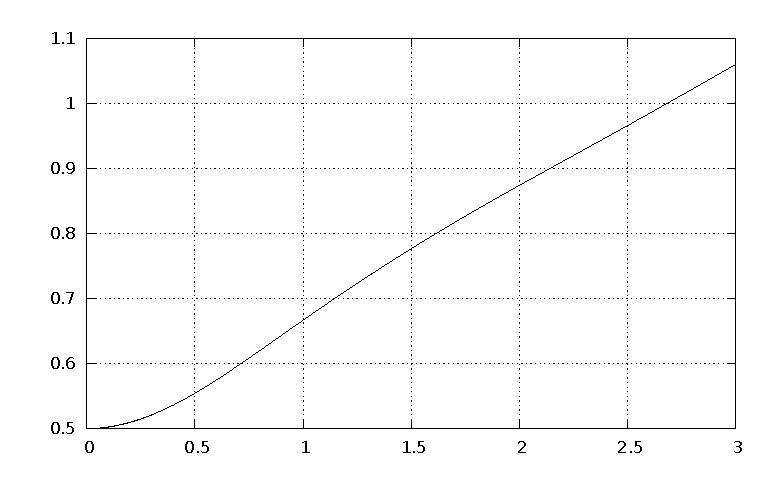
\includegraphics[width=.45\textwidth]
{figures/2d_benchmark1_barycenter_p1p0_128.ps}
\caption{Plot of the centre of mass over time for the simulation with 128 
interface elements and using P2-(P1+P0) element.}
\label{fig:2d_benchmark1_barycenter}
\end{figure}

\begin{figure}[htbp]
\centering
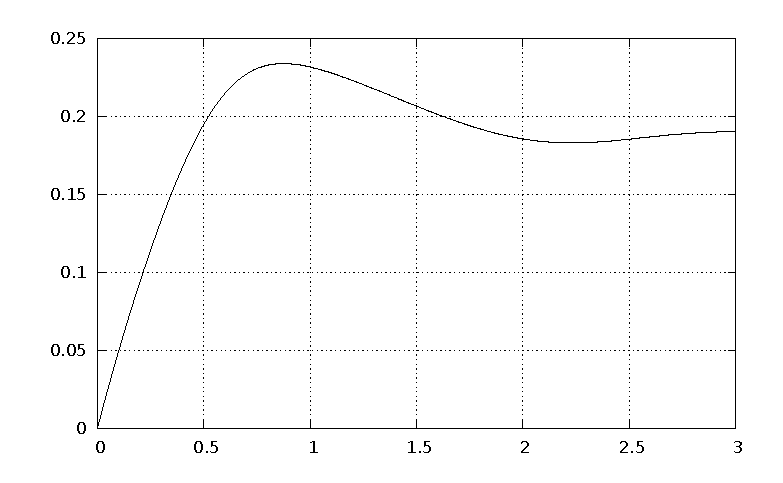
\includegraphics[width=.45\textwidth]
{figures/2d_benchmark1_velocity_p1p0_128.ps}
\caption{Plot of the average rising velocity over time for the simulation 
with 128 interface elements and using P2-(P1+P0) element.}
\label{fig:2d_benchmark1_velocity}
\end{figure}

\begin{figure}[htbp]
\centering
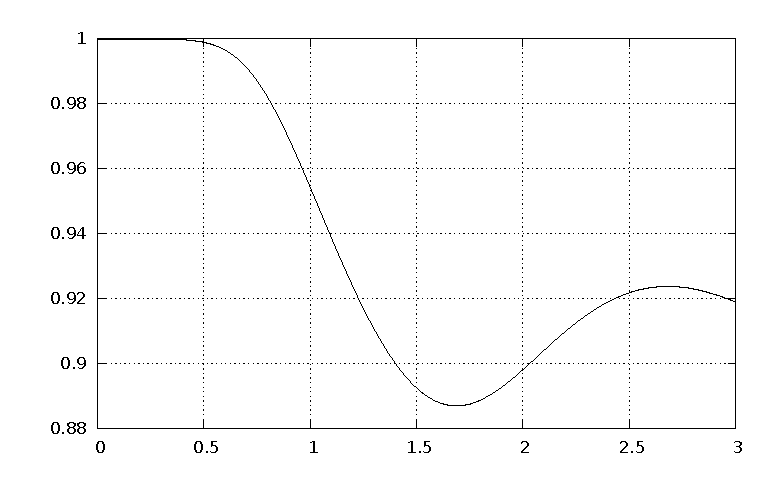
\includegraphics[width=.45\textwidth]
{figures/2d_benchmark1_circularity_p1p0_128.ps}
\caption{Plot of the circularity over time for the simulation with 128 
interface elements and using P2-(P1+P0) element.}
\label{fig:2d_benchmark1_circularity}
\end{figure}

\begin{figure}[htbp]
\centering
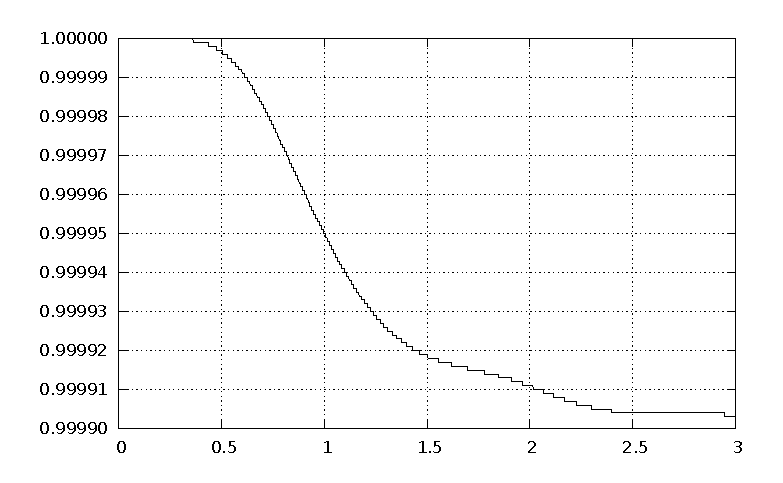
\includegraphics[width=.45\textwidth]
{figures/2d_benchmark1_inner_volume_p1p0_128.ps}
\caption{Plot of the relative inner volume
$\frac{\mathcal{L}^2(\Omega^m_-)}{\mathcal{L}^2(\Omega^0_-)}$ over time for the 
simulation with 128 interface elements and using P2-(P1+P0) element.}
\label{fig:2d_benchmark1_volume}
\end{figure}

\bibliographystyle{siam}
\bibliography{../bib/robert_refs,../bib/marco_refs}
\end{document}